\section{Feature Extraction} \label{sec:features}

We collect 3 types of features from both the DBMS as well as the benchmarking
framework.

\subsection{Features from OLTP-Bench }

  After executing the benchmark, we obtain statistics about the latency and
  throughput delivered by the DBMS.
  This includes both temporal performance metrics as well as aggregate metrics. 
  We then record the size of the workload also known as the
  \textit{scalefactor}.
  The \textit{isolation level} of the DBMS correlates strongly with performance
  metrics Stricter isolation levels like ``serializable level'' correlate with lower
  performance because the DBMS needs to maintain the constraints regarding
  the visibility of effects of concurrent transactions. 
  
  We also record the type
  of DBMS used. Although currently we focus only on Postgres, 
  we anticipate this tool to be useful for other DBMSs as well.   
  We also record the expected label i.e. the benchmark name. This is used for
  evaluating the accuracy of our classification algorithms.  
  
\subsection{Static parameters from Postgres}

  Static parameters are features that do not vary over every execution. This
  primarily includes the configuration parameters of the DBMS and the hardware
  setup.
  For example, these are some of the static parameters that we use as features:\\
   
  \begin{itemize}
    \item {Size of shared memory buffers: This impacts the performance of
    memory-intensive queries significantly.}
    \item {Background writer delay: The background writer issues writes of
    dirty shared buffers to disk. This increases the net overall I/O load but
    allows server processes to avoid waiting for writes to finish.}
    \item {Vacumm cost delay: The vacumm process performs garbage 
    collection. Very short delays can impact the DBMS performance.}
    \item {WAL level: The type of write-ahead logging performed - minimal,
    archive, or hot standby - affects the logging overhead.}
    \item {\textit{fsync}: Durability requirements of data.}
    \item {Sequential page cost: Used in the cost model of the DBMS' planner.}
	\item {Hardware features: CPU cache sizes, DRAM size, disk size, cache latency,
	DRAM latency and disk latency.}
  \end{itemize}
  
  Overall, these metrics significantly impact the performance of the DBMS. A
  non-expert user might not be able to configure these parameters to obtain
  good performance. Our tuning tool can help such users by automatically
  identifying a good DBMS configuration for a given workload.  
  
\subsection{Dynamic parameters from Postgres}
  
  We also collect dynamic parameters from the DBMS during feature extraction.
  To do this, we implemented a Postgres driver that queries the DBMS's internal
  catalog tables like pg\_stat\_database, pg\_statio\_user\_indexes,
  pg\_stat\_activity and pg\_stat\_user\_table
  to obtain useful workload parameters. For instance, these are some of the
  dynamic parameters that we use as features :\\
  
  \begin{itemize}    
    \item {Number of transactions in this database that have been committed or
    rolled back.}
    \item {Number of disk blocks read in this database.}
    \item {Number of times disk blocks were found already in the DBMS's buffer
    cache.}
    \item {Number of rows returned, fetched, inserted, updated or deleted by
    queries in this database.}
    \item {Number of index and cache blocks hit.}
    \item {Status of different storage backends of the DBMS.}
    \item {Size of the tables and indexes in the DBMS.}
    \item {Number of sequential scans and index scans performed by the
    workload.}
  \end{itemize}
  
  	We normalize the relevant metrics by the number of transactions executed.
  	Before the start of an execution, we reset all the statistics using our
  	DBMS driver. Overall, this gives us a nice set of features about the
  	workload. 

\begin{figure*}
    \centering
    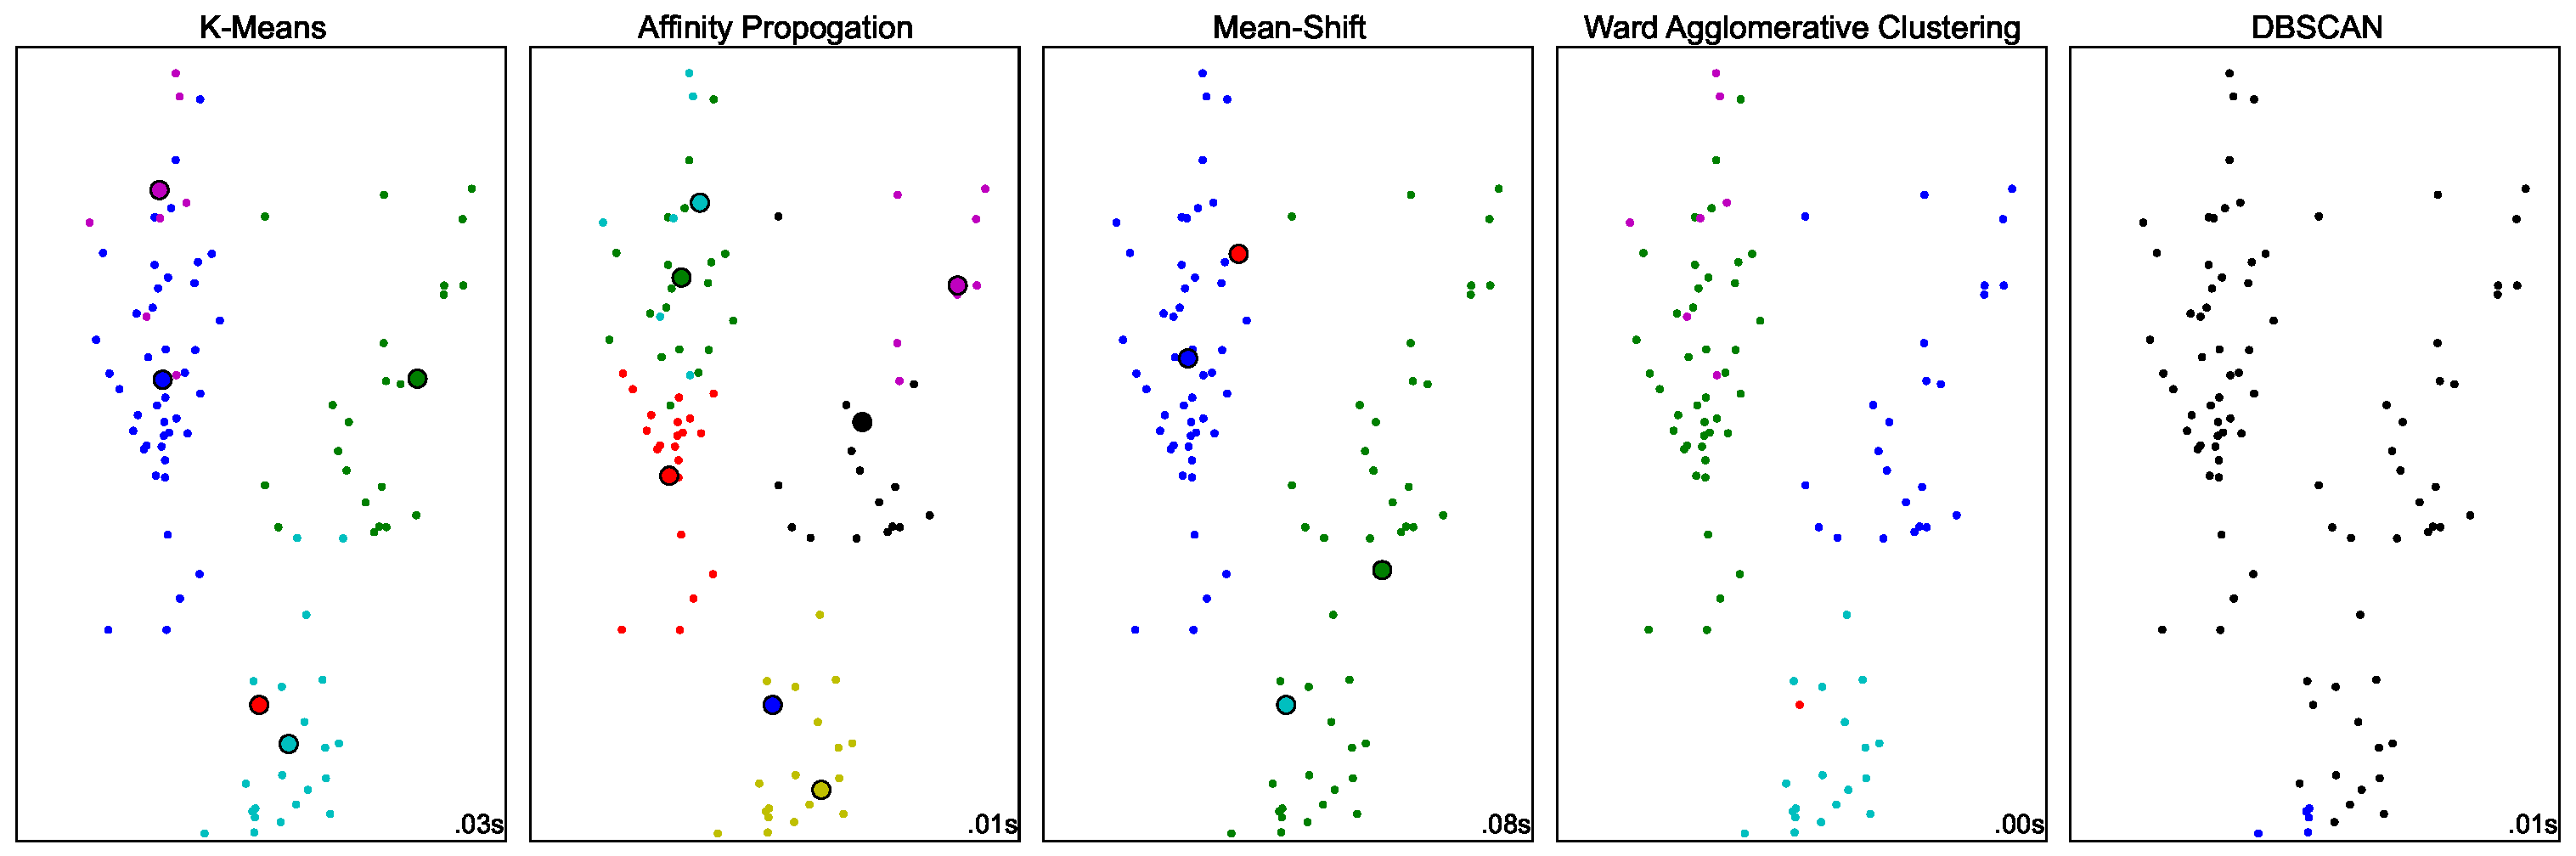
\includegraphics[width=0.95\textwidth]{figure/clustering.eps}
    \caption{Clusters found by the clustering algorithms.}
    \label{fig:clusters}
\end{figure*}

\begin{figure*}[h]
    \centering
    \begin{tabular}{c c c c}
      \toprule
      Algorithm                     & Homogeneity & Completeness & V-Measure \\
      \midrule
      K-Means                       & 1.000       & 1.000        & 1.000     \\
      Affinity-Propagation          & 0.824       & 1.000        & 0.904     \\
      Mean-Shift                    & 1.000       & 0.795        & 0.886     \\
      Ward Agglomerative Clustering & 1.000       & 1.000        & 1.000     \\
      DBSCAN                        & 0.000       & 1.000        & 0.000     \\
      \bottomrule
    \end{tabular}

    \caption{Performance metrics of clustering algorithms.}
    \label{fig:clustering-metrics}
\end{figure*}

After collecting all these features, we transform them to a metric space and
normalize them to generate a feature matrix and a label matrix. This is 
used by the classification algorithms that we describe in the next section.
